% <<< GENERATED FIGURES: scripts/make_figures.py -- do not edit by hand
% Re-run the script instead, or the paper and the data drift apart.
\definecolor{cbBlue}{HTML}{0072B2}
\definecolor{cbOrange}{HTML}{E69F00}
\definecolor{cbGreen}{HTML}{009E73}
\definecolor{cbPurple}{HTML}{CC79A7}
\definecolor{cbRed}{HTML}{D55E00}
\definecolor{cbBrown}{HTML}{8C6D31}

\begin{figure}[t]
\centering
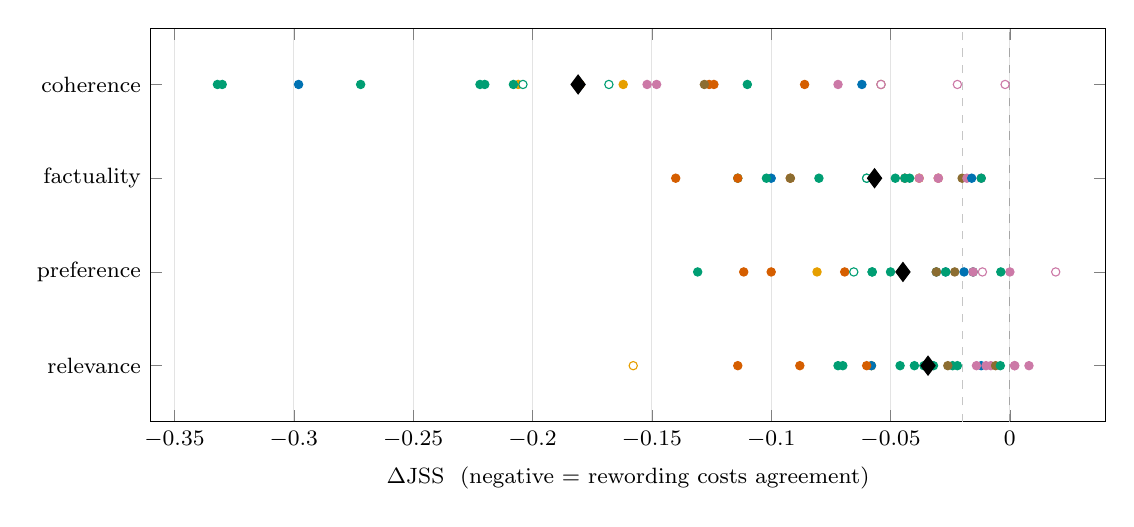
\begin{tikzpicture}
\begin{axis}[
  width=\linewidth, height=5.0cm,
  xlabel={$\Delta\mathrm{JSS}$ \ (negative = rewording costs agreement)},
  xmin=-0.36, xmax=0.04,
  % pgfplots defaults to scientific notation near zero, which collapses the
  % ticks either side of the origin into an unreadable run of 8*10^-2 style
  % labels. Fix the ticks and force plain decimals.
  xtick={-0.35,-0.30,-0.25,-0.20,-0.15,-0.10,-0.05,0},
  scaled x ticks=false,
  x tick label style={/pgf/number format/fixed,
                      /pgf/number format/precision=2},
  ytick={4,3,2,1}, yticklabels={coherence,factuality,preference,relevance},
  ymin=0.4, ymax=4.6,
  xmajorgrids, grid style={gray!22},
  tick label style={font=\footnotesize},
  label style={font=\footnotesize},
  scale only axis,
]
\draw[dashed, gray!70] ({axis cs:0,0}|-{rel axis cs:0,0})
                    -- ({axis cs:0,0}|-{rel axis cs:0,1});
\draw[dashed, gray!45] ({axis cs:-0.02,0}|-{rel axis cs:0,0})
                    -- ({axis cs:-0.02,0}|-{rel axis cs:0,1});
\addplot[only marks, mark=*, mark size=1.5pt, draw=cbOrange, fill=cbOrange] coordinates {(-0.2060,4)};
\addplot[only marks, mark=*, mark size=1.5pt, draw=cbOrange, fill=cbOrange] coordinates {(-0.1800,4)};
\addplot[only marks, mark=*, mark size=1.5pt, draw=cbOrange, fill=cbOrange] coordinates {(-0.1620,4)};
\addplot[only marks, mark=*, mark size=1.5pt, draw=cbPurple, fill=white] coordinates {(-0.0020,4)};
\addplot[only marks, mark=*, mark size=1.5pt, draw=cbBrown, fill=white] coordinates {(-0.0540,4)};
\addplot[only marks, mark=*, mark size=1.5pt, draw=cbPurple, fill=white] coordinates {(-0.0220,4)};
\addplot[only marks, mark=*, mark size=1.5pt, draw=cbBlue, fill=cbBlue] coordinates {(-0.0620,4)};
\addplot[only marks, mark=*, mark size=1.5pt, draw=cbBlue, fill=cbBlue] coordinates {(-0.2980,4)};
\addplot[only marks, mark=*, mark size=1.5pt, draw=cbGreen, fill=cbGreen] coordinates {(-0.1100,4)};
\addplot[only marks, mark=*, mark size=1.5pt, draw=cbPurple, fill=white] coordinates {(-0.0540,4)};
\addplot[only marks, mark=*, mark size=1.5pt, draw=cbPurple, fill=cbPurple] coordinates {(-0.0720,4)};
\addplot[only marks, mark=*, mark size=1.5pt, draw=cbGreen, fill=cbGreen] coordinates {(-0.2200,4)};
\addplot[only marks, mark=*, mark size=1.5pt, draw=cbGreen, fill=cbGreen] coordinates {(-0.2220,4)};
\addplot[only marks, mark=*, mark size=1.5pt, draw=cbGreen, fill=cbGreen] coordinates {(-0.3300,4)};
\addplot[only marks, mark=*, mark size=1.5pt, draw=cbGreen, fill=cbGreen] coordinates {(-0.3320,4)};
\addplot[only marks, mark=*, mark size=1.5pt, draw=cbRed, fill=cbRed] coordinates {(-0.1240,4)};
\addplot[only marks, mark=*, mark size=1.5pt, draw=cbRed, fill=cbRed] coordinates {(-0.0860,4)};
\addplot[only marks, mark=*, mark size=1.5pt, draw=cbRed, fill=cbRed] coordinates {(-0.1260,4)};
\addplot[only marks, mark=*, mark size=1.5pt, draw=cbPurple, fill=cbPurple] coordinates {(-0.1520,4)};
\addplot[only marks, mark=*, mark size=1.5pt, draw=cbGreen, fill=white] coordinates {(-0.2040,4)};
\addplot[only marks, mark=*, mark size=1.5pt, draw=cbGreen, fill=cbGreen] coordinates {(-0.2720,4)};
\addplot[only marks, mark=*, mark size=1.5pt, draw=cbGreen, fill=white] coordinates {(-0.1680,4)};
\addplot[only marks, mark=*, mark size=1.5pt, draw=cbPurple, fill=cbPurple] coordinates {(-0.1480,4)};
\addplot[only marks, mark=*, mark size=1.5pt, draw=cbGreen, fill=cbGreen] coordinates {(-0.2080,4)};
\addplot[only marks, mark=*, mark size=1.5pt, draw=cbBrown, fill=cbBrown] coordinates {(-0.1280,4)};
\addplot[only marks, mark=diamond*, mark size=3.4pt, draw=black, fill=black] coordinates {(-0.1809,4)};
\addplot[only marks, mark=*, mark size=1.5pt, draw=cbOrange, fill=cbOrange] coordinates {(-0.0440,3)};
\addplot[only marks, mark=*, mark size=1.5pt, draw=cbOrange, fill=cbOrange] coordinates {(-0.0300,3)};
\addplot[only marks, mark=*, mark size=1.5pt, draw=cbOrange, fill=cbOrange] coordinates {(-0.0380,3)};
\addplot[only marks, mark=*, mark size=1.5pt, draw=cbPurple, fill=cbPurple] coordinates {(-0.0120,3)};
\addplot[only marks, mark=*, mark size=1.5pt, draw=cbBrown, fill=cbBrown] coordinates {(-0.0200,3)};
\addplot[only marks, mark=*, mark size=1.5pt, draw=cbPurple, fill=cbPurple] coordinates {(-0.0180,3)};
\addplot[only marks, mark=*, mark size=1.5pt, draw=cbBlue, fill=cbBlue] coordinates {(-0.0160,3)};
\addplot[only marks, mark=*, mark size=1.5pt, draw=cbBlue, fill=cbBlue] coordinates {(-0.1000,3)};
\addplot[only marks, mark=*, mark size=1.5pt, draw=cbGreen, fill=cbGreen] coordinates {(-0.0120,3)};
\addplot[only marks, mark=*, mark size=1.5pt, draw=cbPurple, fill=cbPurple] coordinates {(-0.0300,3)};
\addplot[only marks, mark=*, mark size=1.5pt, draw=cbPurple, fill=cbPurple] coordinates {(-0.0440,3)};
\addplot[only marks, mark=*, mark size=1.5pt, draw=cbGreen, fill=cbGreen] coordinates {(-0.0480,3)};
\addplot[only marks, mark=*, mark size=1.5pt, draw=cbGreen, fill=cbGreen] coordinates {(-0.0800,3)};
\addplot[only marks, mark=*, mark size=1.5pt, draw=cbGreen, fill=cbGreen] coordinates {(-0.1020,3)};
\addplot[only marks, mark=*, mark size=1.5pt, draw=cbGreen, fill=cbGreen] coordinates {(-0.1140,3)};
\addplot[only marks, mark=*, mark size=1.5pt, draw=cbRed, fill=cbRed] coordinates {(-0.1400,3)};
\addplot[only marks, mark=*, mark size=1.5pt, draw=cbRed, fill=cbRed] coordinates {(-0.0920,3)};
\addplot[only marks, mark=*, mark size=1.5pt, draw=cbRed, fill=cbRed] coordinates {(-0.1140,3)};
\addplot[only marks, mark=*, mark size=1.5pt, draw=cbPurple, fill=cbPurple] coordinates {(-0.0380,3)};
\addplot[only marks, mark=*, mark size=1.5pt, draw=cbGreen, fill=cbGreen] coordinates {(-0.0420,3)};
\addplot[only marks, mark=*, mark size=1.5pt, draw=cbGreen, fill=cbGreen] coordinates {(-0.0440,3)};
\addplot[only marks, mark=*, mark size=1.5pt, draw=cbGreen, fill=cbGreen] coordinates {(-0.0600,3)};
\addplot[only marks, mark=*, mark size=1.5pt, draw=cbPurple, fill=cbPurple] coordinates {(-0.0300,3)};
\addplot[only marks, mark=*, mark size=1.5pt, draw=cbGreen, fill=white] coordinates {(-0.0600,3)};
\addplot[only marks, mark=*, mark size=1.5pt, draw=cbBrown, fill=cbBrown] coordinates {(-0.0920,3)};
\addplot[only marks, mark=diamond*, mark size=3.4pt, draw=black, fill=black] coordinates {(-0.0567,3)};
\addplot[only marks, mark=*, mark size=1.5pt, draw=cbOrange, fill=cbOrange] coordinates {(-0.0808,2)};
\addplot[only marks, mark=*, mark size=1.5pt, draw=cbPurple, fill=cbPurple] coordinates {(0.0000,2)};
\addplot[only marks, mark=*, mark size=1.5pt, draw=cbBrown, fill=cbBrown] coordinates {(-0.0231,2)};
\addplot[only marks, mark=*, mark size=1.5pt, draw=cbPurple, fill=white] coordinates {(0.0192,2)};
\addplot[only marks, mark=*, mark size=1.5pt, draw=cbBlue, fill=cbBlue] coordinates {(-0.0192,2)};
\addplot[only marks, mark=*, mark size=1.5pt, draw=cbBlue, fill=cbBlue] coordinates {(-0.0269,2)};
\addplot[only marks, mark=*, mark size=1.5pt, draw=cbGreen, fill=cbGreen] coordinates {(-0.0038,2)};
\addplot[only marks, mark=*, mark size=1.5pt, draw=cbPurple, fill=white] coordinates {(-0.0115,2)};
\addplot[only marks, mark=*, mark size=1.5pt, draw=cbPurple, fill=cbPurple] coordinates {(-0.0154,2)};
\addplot[only marks, mark=*, mark size=1.5pt, draw=cbGreen, fill=cbGreen] coordinates {(-0.0154,2)};
\addplot[only marks, mark=*, mark size=1.5pt, draw=cbGreen, fill=cbGreen] coordinates {(-0.0577,2)};
\addplot[only marks, mark=*, mark size=1.5pt, draw=cbGreen, fill=cbGreen] coordinates {(-0.1308,2)};
\addplot[only marks, mark=*, mark size=1.5pt, draw=cbGreen, fill=cbGreen] coordinates {(-0.0577,2)};
\addplot[only marks, mark=*, mark size=1.5pt, draw=cbRed, fill=cbRed] coordinates {(-0.1115,2)};
\addplot[only marks, mark=*, mark size=1.5pt, draw=cbRed, fill=cbRed] coordinates {(-0.0692,2)};
\addplot[only marks, mark=*, mark size=1.5pt, draw=cbRed, fill=cbRed] coordinates {(-0.1000,2)};
\addplot[only marks, mark=*, mark size=1.5pt, draw=cbPurple, fill=cbPurple] coordinates {(-0.0308,2)};
\addplot[only marks, mark=*, mark size=1.5pt, draw=cbGreen, fill=cbGreen] coordinates {(-0.0500,2)};
\addplot[only marks, mark=*, mark size=1.5pt, draw=cbGreen, fill=cbGreen] coordinates {(-0.0269,2)};
\addplot[only marks, mark=*, mark size=1.5pt, draw=cbGreen, fill=white] coordinates {(-0.0654,2)};
\addplot[only marks, mark=*, mark size=1.5pt, draw=cbPurple, fill=cbPurple] coordinates {(-0.0154,2)};
\addplot[only marks, mark=*, mark size=1.5pt, draw=cbGreen, fill=cbGreen] coordinates {(-0.0308,2)};
\addplot[only marks, mark=*, mark size=1.5pt, draw=cbBrown, fill=cbBrown] coordinates {(-0.0308,2)};
\addplot[only marks, mark=diamond*, mark size=3.4pt, draw=black, fill=black] coordinates {(-0.0448,2)};
\addplot[only marks, mark=*, mark size=1.5pt, draw=cbOrange, fill=cbOrange] coordinates {(-0.0580,1)};
\addplot[only marks, mark=*, mark size=1.5pt, draw=cbOrange, fill=cbOrange] coordinates {(-0.0357,1)};
\addplot[only marks, mark=*, mark size=1.5pt, draw=cbOrange, fill=white] coordinates {(-0.1578,1)};
\addplot[only marks, mark=*, mark size=1.5pt, draw=cbPurple, fill=cbPurple] coordinates {(-0.0080,1)};
\addplot[only marks, mark=*, mark size=1.5pt, draw=cbBrown, fill=cbBrown] coordinates {(-0.0060,1)};
\addplot[only marks, mark=*, mark size=1.5pt, draw=cbPurple, fill=cbPurple] coordinates {(0.0080,1)};
\addplot[only marks, mark=*, mark size=1.5pt, draw=cbBlue, fill=cbBlue] coordinates {(-0.0120,1)};
\addplot[only marks, mark=*, mark size=1.5pt, draw=cbBlue, fill=cbBlue] coordinates {(-0.0580,1)};
\addplot[only marks, mark=*, mark size=1.5pt, draw=cbGreen, fill=cbGreen] coordinates {(-0.0400,1)};
\addplot[only marks, mark=*, mark size=1.5pt, draw=cbPurple, fill=cbPurple] coordinates {(0.0020,1)};
\addplot[only marks, mark=*, mark size=1.5pt, draw=cbPurple, fill=cbPurple] coordinates {(-0.0140,1)};
\addplot[only marks, mark=*, mark size=1.5pt, draw=cbGreen, fill=cbGreen] coordinates {(-0.0460,1)};
\addplot[only marks, mark=*, mark size=1.5pt, draw=cbGreen, fill=cbGreen] coordinates {(-0.0220,1)};
\addplot[only marks, mark=*, mark size=1.5pt, draw=cbGreen, fill=cbGreen] coordinates {(-0.0700,1)};
\addplot[only marks, mark=*, mark size=1.5pt, draw=cbGreen, fill=cbGreen] coordinates {(-0.0720,1)};
\addplot[only marks, mark=*, mark size=1.5pt, draw=cbRed, fill=cbRed] coordinates {(-0.0880,1)};
\addplot[only marks, mark=*, mark size=1.5pt, draw=cbRed, fill=cbRed] coordinates {(-0.0600,1)};
\addplot[only marks, mark=*, mark size=1.5pt, draw=cbRed, fill=cbRed] coordinates {(-0.1140,1)};
\addplot[only marks, mark=*, mark size=1.5pt, draw=cbPurple, fill=cbPurple] coordinates {(0.0020,1)};
\addplot[only marks, mark=*, mark size=1.5pt, draw=cbGreen, fill=cbGreen] coordinates {(-0.0040,1)};
\addplot[only marks, mark=*, mark size=1.5pt, draw=cbGreen, fill=cbGreen] coordinates {(-0.0360,1)};
\addplot[only marks, mark=*, mark size=1.5pt, draw=cbGreen, fill=cbGreen] coordinates {(-0.0320,1)};
\addplot[only marks, mark=*, mark size=1.5pt, draw=cbPurple, fill=cbPurple] coordinates {(-0.0100,1)};
\addplot[only marks, mark=*, mark size=1.5pt, draw=cbGreen, fill=cbGreen] coordinates {(-0.0240,1)};
\addplot[only marks, mark=*, mark size=1.5pt, draw=cbBrown, fill=cbBrown] coordinates {(-0.0260,1)};
\addplot[only marks, mark=diamond*, mark size=3.4pt, draw=black, fill=black] coordinates {(-0.0343,1)};
\end{axis}
\end{tikzpicture}
\caption{\textbf{Paraphrase cost by task across twenty-five judges.} One marker
per judge--task cell, coloured by provider; hollow markers are the eleven cells
whose repeat ceiling falls below $0.90$ and which we decline to read; black
diamonds are the pooled mean per task. Dashed lines mark zero and the $-0.02$
smallest effect of interest. Takeaway: the cost is negative almost everywhere,
coherence is both the largest loss and by far the widest spread across judges,
and the three same-vendor judges of the superseded version sit close together,
which is what produced its retracted claim that the task matters more than the
judge.}
\label{fig:delta}
\end{figure}

\begin{figure}[t]
\centering
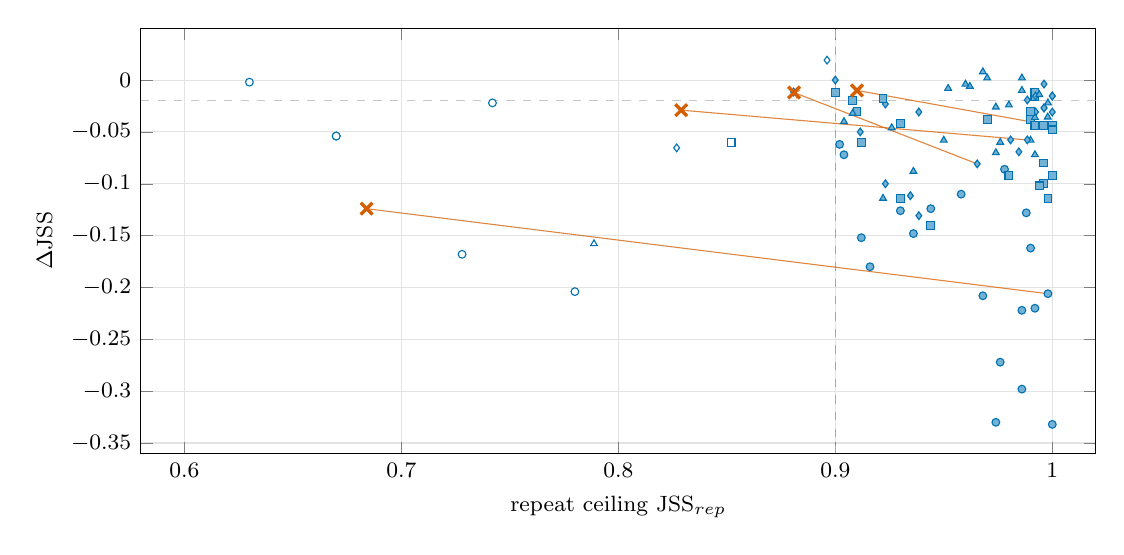
\begin{tikzpicture}
\begin{axis}[
  width=\linewidth, height=5.4cm,
  xlabel={repeat ceiling $\mathrm{JSS}_{\text{rep}}$},
  ylabel={$\Delta\mathrm{JSS}$},
  xmin=0.58, xmax=1.02, ymin=-0.36, ymax=0.05,
  xtick={0.6,0.7,0.8,0.9,1.0},
  ytick={-0.35,-0.30,-0.25,-0.20,-0.15,-0.10,-0.05,0},
  scaled ticks=false,
  tick label style={/pgf/number format/fixed,
                    /pgf/number format/precision=2, font=\footnotesize},
  xmajorgrids, ymajorgrids, grid style={gray!22},
  label style={font=\footnotesize},
  scale only axis,
]
\draw[dashed, gray!70] (axis cs:0.90,-0.36) -- (axis cs:0.90,0.05);
\draw[dashed, gray!45] (axis cs:0.58,-0.02) -- (axis cs:1.02,-0.02);
\addplot[only marks, mark=*, mark size=1.4pt, draw=cbBlue, fill=cbBlue!55] coordinates {(0.9980,-0.2060)};
\addplot[only marks, mark=square*, mark size=1.4pt, draw=cbBlue, fill=cbBlue!55] coordinates {(1.0000,-0.0440)};
\addplot[only marks, mark=diamond*, mark size=1.4pt, draw=cbBlue, fill=cbBlue!55] coordinates {(0.9654,-0.0808)};
\addplot[only marks, mark=triangle*, mark size=1.4pt, draw=cbBlue, fill=cbBlue!55] coordinates {(0.9900,-0.0580)};
\addplot[only marks, mark=*, mark size=1.4pt, draw=cbBlue, fill=cbBlue!55] coordinates {(0.9160,-0.1800)};
\addplot[only marks, mark=square*, mark size=1.4pt, draw=cbBlue, fill=cbBlue!55] coordinates {(0.9900,-0.0300)};
\addplot[only marks, mark=triangle*, mark size=1.4pt, draw=cbBlue, fill=cbBlue!55] coordinates {(0.9979,-0.0357)};
\addplot[only marks, mark=*, mark size=1.4pt, draw=cbBlue, fill=cbBlue!55] coordinates {(0.9900,-0.1620)};
\addplot[only marks, mark=square*, mark size=1.4pt, draw=cbBlue, fill=cbBlue!55] coordinates {(0.9900,-0.0380)};
\addplot[only marks, mark=triangle*, mark size=1.4pt, draw=cbBlue, fill=white] coordinates {(0.7888,-0.1578)};
\addplot[only marks, mark=*, mark size=1.4pt, draw=cbBlue, fill=white] coordinates {(0.6300,-0.0020)};
\addplot[only marks, mark=square*, mark size=1.4pt, draw=cbBlue, fill=cbBlue!55] coordinates {(0.9000,-0.0120)};
\addplot[only marks, mark=diamond*, mark size=1.4pt, draw=cbBlue, fill=cbBlue!55] coordinates {(0.9000,0.0000)};
\addplot[only marks, mark=triangle*, mark size=1.4pt, draw=cbBlue, fill=cbBlue!55] coordinates {(0.9520,-0.0080)};
\addplot[only marks, mark=*, mark size=1.4pt, draw=cbBlue, fill=white] coordinates {(0.6700,-0.0540)};
\addplot[only marks, mark=square*, mark size=1.4pt, draw=cbBlue, fill=cbBlue!55] coordinates {(0.9080,-0.0200)};
\addplot[only marks, mark=diamond*, mark size=1.4pt, draw=cbBlue, fill=cbBlue!55] coordinates {(0.9231,-0.0231)};
\addplot[only marks, mark=triangle*, mark size=1.4pt, draw=cbBlue, fill=cbBlue!55] coordinates {(0.9620,-0.0060)};
\addplot[only marks, mark=*, mark size=1.4pt, draw=cbBlue, fill=white] coordinates {(0.7420,-0.0220)};
\addplot[only marks, mark=square*, mark size=1.4pt, draw=cbBlue, fill=cbBlue!55] coordinates {(0.9220,-0.0180)};
\addplot[only marks, mark=diamond*, mark size=1.4pt, draw=cbBlue, fill=white] coordinates {(0.8962,0.0192)};
\addplot[only marks, mark=triangle*, mark size=1.4pt, draw=cbBlue, fill=cbBlue!55] coordinates {(0.9680,0.0080)};
\addplot[only marks, mark=*, mark size=1.4pt, draw=cbBlue, fill=cbBlue!55] coordinates {(0.9020,-0.0620)};
\addplot[only marks, mark=square*, mark size=1.4pt, draw=cbBlue, fill=cbBlue!55] coordinates {(0.9920,-0.0160)};
\addplot[only marks, mark=diamond*, mark size=1.4pt, draw=cbBlue, fill=cbBlue!55] coordinates {(0.9885,-0.0192)};
\addplot[only marks, mark=triangle*, mark size=1.4pt, draw=cbBlue, fill=cbBlue!55] coordinates {(0.9920,-0.0120)};
\addplot[only marks, mark=*, mark size=1.4pt, draw=cbBlue, fill=cbBlue!55] coordinates {(0.9860,-0.2980)};
\addplot[only marks, mark=square*, mark size=1.4pt, draw=cbBlue, fill=cbBlue!55] coordinates {(0.9960,-0.1000)};
\addplot[only marks, mark=diamond*, mark size=1.4pt, draw=cbBlue, fill=cbBlue!55] coordinates {(0.9962,-0.0269)};
\addplot[only marks, mark=triangle*, mark size=1.4pt, draw=cbBlue, fill=cbBlue!55] coordinates {(0.9500,-0.0580)};
\addplot[only marks, mark=*, mark size=1.4pt, draw=cbBlue, fill=cbBlue!55] coordinates {(0.9580,-0.1100)};
\addplot[only marks, mark=square*, mark size=1.4pt, draw=cbBlue, fill=cbBlue!55] coordinates {(0.9920,-0.0120)};
\addplot[only marks, mark=diamond*, mark size=1.4pt, draw=cbBlue, fill=cbBlue!55] coordinates {(0.9962,-0.0038)};
\addplot[only marks, mark=triangle*, mark size=1.4pt, draw=cbBlue, fill=cbBlue!55] coordinates {(0.9040,-0.0400)};
\addplot[only marks, mark=*, mark size=1.4pt, draw=cbBlue, fill=white] coordinates {(0.6700,-0.0540)};
\addplot[only marks, mark=square*, mark size=1.4pt, draw=cbBlue, fill=cbBlue!55] coordinates {(0.9100,-0.0300)};
\addplot[only marks, mark=diamond*, mark size=1.4pt, draw=cbBlue, fill=white] coordinates {(0.8808,-0.0115)};
\addplot[only marks, mark=triangle*, mark size=1.4pt, draw=cbBlue, fill=cbBlue!55] coordinates {(0.9700,0.0020)};
\addplot[only marks, mark=*, mark size=1.4pt, draw=cbBlue, fill=cbBlue!55] coordinates {(0.9040,-0.0720)};
\addplot[only marks, mark=square*, mark size=1.4pt, draw=cbBlue, fill=cbBlue!55] coordinates {(0.9920,-0.0440)};
\addplot[only marks, mark=diamond*, mark size=1.4pt, draw=cbBlue, fill=cbBlue!55] coordinates {(0.9923,-0.0154)};
\addplot[only marks, mark=triangle*, mark size=1.4pt, draw=cbBlue, fill=cbBlue!55] coordinates {(0.9940,-0.0140)};
\addplot[only marks, mark=*, mark size=1.4pt, draw=cbBlue, fill=cbBlue!55] coordinates {(0.9920,-0.2200)};
\addplot[only marks, mark=square*, mark size=1.4pt, draw=cbBlue, fill=cbBlue!55] coordinates {(1.0000,-0.0480)};
\addplot[only marks, mark=diamond*, mark size=1.4pt, draw=cbBlue, fill=cbBlue!55] coordinates {(1.0000,-0.0154)};
\addplot[only marks, mark=triangle*, mark size=1.4pt, draw=cbBlue, fill=cbBlue!55] coordinates {(0.9260,-0.0460)};
\addplot[only marks, mark=*, mark size=1.4pt, draw=cbBlue, fill=cbBlue!55] coordinates {(0.9860,-0.2220)};
\addplot[only marks, mark=square*, mark size=1.4pt, draw=cbBlue, fill=cbBlue!55] coordinates {(0.9960,-0.0800)};
\addplot[only marks, mark=diamond*, mark size=1.4pt, draw=cbBlue, fill=cbBlue!55] coordinates {(0.9885,-0.0577)};
\addplot[only marks, mark=triangle*, mark size=1.4pt, draw=cbBlue, fill=cbBlue!55] coordinates {(0.9980,-0.0220)};
\addplot[only marks, mark=*, mark size=1.4pt, draw=cbBlue, fill=cbBlue!55] coordinates {(0.9740,-0.3300)};
\addplot[only marks, mark=square*, mark size=1.4pt, draw=cbBlue, fill=cbBlue!55] coordinates {(0.9940,-0.1020)};
\addplot[only marks, mark=diamond*, mark size=1.4pt, draw=cbBlue, fill=cbBlue!55] coordinates {(0.9385,-0.1308)};
\addplot[only marks, mark=triangle*, mark size=1.4pt, draw=cbBlue, fill=cbBlue!55] coordinates {(0.9740,-0.0700)};
\addplot[only marks, mark=*, mark size=1.4pt, draw=cbBlue, fill=cbBlue!55] coordinates {(1.0000,-0.3320)};
\addplot[only marks, mark=square*, mark size=1.4pt, draw=cbBlue, fill=cbBlue!55] coordinates {(0.9980,-0.1140)};
\addplot[only marks, mark=diamond*, mark size=1.4pt, draw=cbBlue, fill=cbBlue!55] coordinates {(0.9808,-0.0577)};
\addplot[only marks, mark=triangle*, mark size=1.4pt, draw=cbBlue, fill=cbBlue!55] coordinates {(0.9920,-0.0720)};
\addplot[only marks, mark=*, mark size=1.4pt, draw=cbBlue, fill=cbBlue!55] coordinates {(0.9440,-0.1240)};
\addplot[only marks, mark=square*, mark size=1.4pt, draw=cbBlue, fill=cbBlue!55] coordinates {(0.9440,-0.1400)};
\addplot[only marks, mark=diamond*, mark size=1.4pt, draw=cbBlue, fill=cbBlue!55] coordinates {(0.9346,-0.1115)};
\addplot[only marks, mark=triangle*, mark size=1.4pt, draw=cbBlue, fill=cbBlue!55] coordinates {(0.9360,-0.0880)};
\addplot[only marks, mark=*, mark size=1.4pt, draw=cbBlue, fill=cbBlue!55] coordinates {(0.9780,-0.0860)};
\addplot[only marks, mark=square*, mark size=1.4pt, draw=cbBlue, fill=cbBlue!55] coordinates {(0.9800,-0.0920)};
\addplot[only marks, mark=diamond*, mark size=1.4pt, draw=cbBlue, fill=cbBlue!55] coordinates {(0.9846,-0.0692)};
\addplot[only marks, mark=triangle*, mark size=1.4pt, draw=cbBlue, fill=cbBlue!55] coordinates {(0.9760,-0.0600)};
\addplot[only marks, mark=*, mark size=1.4pt, draw=cbBlue, fill=cbBlue!55] coordinates {(0.9300,-0.1260)};
\addplot[only marks, mark=square*, mark size=1.4pt, draw=cbBlue, fill=cbBlue!55] coordinates {(0.9300,-0.1140)};
\addplot[only marks, mark=diamond*, mark size=1.4pt, draw=cbBlue, fill=cbBlue!55] coordinates {(0.9231,-0.1000)};
\addplot[only marks, mark=triangle*, mark size=1.4pt, draw=cbBlue, fill=cbBlue!55] coordinates {(0.9220,-0.1140)};
\addplot[only marks, mark=*, mark size=1.4pt, draw=cbBlue, fill=cbBlue!55] coordinates {(0.9120,-0.1520)};
\addplot[only marks, mark=square*, mark size=1.4pt, draw=cbBlue, fill=cbBlue!55] coordinates {(0.9700,-0.0380)};
\addplot[only marks, mark=diamond*, mark size=1.4pt, draw=cbBlue, fill=cbBlue!55] coordinates {(0.9923,-0.0308)};
\addplot[only marks, mark=triangle*, mark size=1.4pt, draw=cbBlue, fill=cbBlue!55] coordinates {(0.9860,0.0020)};
\addplot[only marks, mark=*, mark size=1.4pt, draw=cbBlue, fill=white] coordinates {(0.7800,-0.2040)};
\addplot[only marks, mark=square*, mark size=1.4pt, draw=cbBlue, fill=cbBlue!55] coordinates {(0.9300,-0.0420)};
\addplot[only marks, mark=diamond*, mark size=1.4pt, draw=cbBlue, fill=cbBlue!55] coordinates {(0.9115,-0.0500)};
\addplot[only marks, mark=triangle*, mark size=1.4pt, draw=cbBlue, fill=cbBlue!55] coordinates {(0.9600,-0.0040)};
\addplot[only marks, mark=*, mark size=1.4pt, draw=cbBlue, fill=cbBlue!55] coordinates {(0.9760,-0.2720)};
\addplot[only marks, mark=square*, mark size=1.4pt, draw=cbBlue, fill=cbBlue!55] coordinates {(0.9960,-0.0440)};
\addplot[only marks, mark=diamond*, mark size=1.4pt, draw=cbBlue, fill=cbBlue!55] coordinates {(0.9962,-0.0269)};
\addplot[only marks, mark=triangle*, mark size=1.4pt, draw=cbBlue, fill=cbBlue!55] coordinates {(0.9920,-0.0360)};
\addplot[only marks, mark=*, mark size=1.4pt, draw=cbBlue, fill=white] coordinates {(0.7280,-0.1680)};
\addplot[only marks, mark=square*, mark size=1.4pt, draw=cbBlue, fill=cbBlue!55] coordinates {(0.9120,-0.0600)};
\addplot[only marks, mark=diamond*, mark size=1.4pt, draw=cbBlue, fill=white] coordinates {(0.8269,-0.0654)};
\addplot[only marks, mark=triangle*, mark size=1.4pt, draw=cbBlue, fill=cbBlue!55] coordinates {(0.9080,-0.0320)};
\addplot[only marks, mark=*, mark size=1.4pt, draw=cbBlue, fill=cbBlue!55] coordinates {(0.9360,-0.1480)};
\addplot[only marks, mark=square*, mark size=1.4pt, draw=cbBlue, fill=cbBlue!55] coordinates {(0.9900,-0.0300)};
\addplot[only marks, mark=diamond*, mark size=1.4pt, draw=cbBlue, fill=cbBlue!55] coordinates {(1.0000,-0.0154)};
\addplot[only marks, mark=triangle*, mark size=1.4pt, draw=cbBlue, fill=cbBlue!55] coordinates {(0.9860,-0.0100)};
\addplot[only marks, mark=*, mark size=1.4pt, draw=cbBlue, fill=cbBlue!55] coordinates {(0.9680,-0.2080)};
\addplot[only marks, mark=square*, mark size=1.4pt, draw=cbBlue, fill=white] coordinates {(0.8520,-0.0600)};
\addplot[only marks, mark=diamond*, mark size=1.4pt, draw=cbBlue, fill=cbBlue!55] coordinates {(0.9385,-0.0308)};
\addplot[only marks, mark=triangle*, mark size=1.4pt, draw=cbBlue, fill=cbBlue!55] coordinates {(0.9800,-0.0240)};
\addplot[only marks, mark=*, mark size=1.4pt, draw=cbBlue, fill=cbBlue!55] coordinates {(0.9880,-0.1280)};
\addplot[only marks, mark=square*, mark size=1.4pt, draw=cbBlue, fill=cbBlue!55] coordinates {(1.0000,-0.0920)};
\addplot[only marks, mark=diamond*, mark size=1.4pt, draw=cbBlue, fill=cbBlue!55] coordinates {(1.0000,-0.0308)};
\addplot[only marks, mark=triangle*, mark size=1.4pt, draw=cbBlue, fill=cbBlue!55] coordinates {(0.9740,-0.0260)};
\addplot[only marks, mark=x, mark size=3pt, draw=cbRed, very thick] coordinates {(0.6840,-0.1240)};
\addplot[only marks, mark=x, mark size=3pt, draw=cbRed, very thick] coordinates {(0.9100,-0.0100)};
\addplot[only marks, mark=x, mark size=3pt, draw=cbRed, very thick] coordinates {(0.8810,-0.0120)};
\addplot[only marks, mark=x, mark size=3pt, draw=cbRed, very thick] coordinates {(0.8290,-0.0290)};
\draw[->, cbRed, thin, opacity=0.75] (axis cs:0.9980,-0.2060) -- (axis cs:0.6840,-0.1240);
\draw[->, cbRed, thin, opacity=0.75] (axis cs:1.0000,-0.0440) -- (axis cs:0.9100,-0.0100);
\draw[->, cbRed, thin, opacity=0.75] (axis cs:0.9654,-0.0808) -- (axis cs:0.8810,-0.0120);
\draw[->, cbRed, thin, opacity=0.75] (axis cs:0.9900,-0.0580) -- (axis cs:0.8290,-0.0290);
\end{axis}
\end{tikzpicture}
\caption{\textbf{Repeat ceiling against paraphrase cost, all ninety-eight cells,
with the agent-harness cells overlaid.} Marker shape gives the task; hollow
markers fall left of the $0.90$ readability bar. Red crosses are Haiku measured
through the agent harness, joined by arrows to the same judge and task measured
through a direct API call. Takeaway: a low ceiling pulls $\Delta\mathrm{JSS}$
toward zero rather than away from it, so uncontrolled decoding hides wording
sensitivity instead of exposing it, and the harness arrows move left and up for
exactly that reason.}
\label{fig:ceiling}
\end{figure}
